Følgende er baseret på \cite[pp. 27-38]{rose2012software}.

I følge Sarasvathy er der to paradigmer indenfor entrepenørskab.
Disse gør sig også gældende indenfor software entrepenørskab.
De to paradigmer, ADE og CDA, agerer poler, på samme måde som traditionel og agil software udvikling.

Det første af de to paradigmer er ADE:\\
\begin{center}
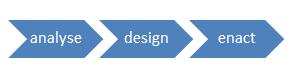
\includegraphics[width=.5\textwidth]{graphics/ade}
\end{center}

ADE minder i høj grad om traditionel software udvikling, idet der forsøges at planlægges og designes således der vil forekomme færre uforudsete problemer.

I modsætning til ADE vil CDA ikke forudsige, men nærmere forsøge at kontrollere.
Dette er en iterativ proces, i stil med agil software udvikling:\\
\begin{center}
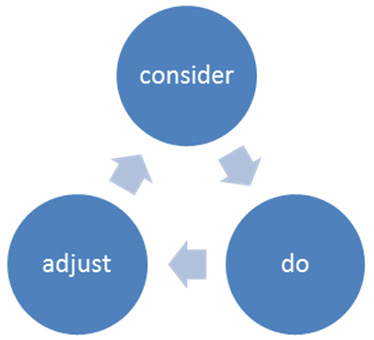
\includegraphics[width=.5\textwidth]{graphics/cda}
\end{center}

Som \citet{rose2012software} nævner vil de fleste organisationer falde under begge paradigmer.
Dette ser vi umiddelbart også som værende tilfældet for vores forretning, hvorfor vi systematisk vil gennemgå sammenligningstabellen i \citet[p. 38]{rose2012software}.

\paragraph{Process:}I første omgang vil der vælges en sekventiel tilgang, da vi har hardware og software der skal laves og begge disse er meget sikkerhedskritiske.
Det menes derfor at det kunne være kritisk at få et ufærdigt produkt ud, da tilliden til vores forretning er vigtig.
Efter første udrulning vil der derimod kunne indføres en mere iterativ tilgang, når først vi har vundet den tillid.

\paragraph{Understanding of future:}
Vi vil gerne styre fremtiden, altså sætte en høj standard for sikkerhed som andre vil få svært ved at følge.
På denne måde skal vi være gode til at tilpasse os, så vores produkt følger med til de stigende/ændrede generelle sikkerhedskrav.

\paragraph{Attitude to market:} Vores produkt er som sådan ikke nyt, da der allerede findes adskillige måder at håndtere passwords og deling af passwords.
Vi forsøger derimod at skabe et nyt marked, ved at bringe et kombineret sikkerhedsprodukt til virksomheder, hvor de måske ikke er klar over at de har brug for det.

\paragraph{Attitude to technology development:}
Vi vil gerne være foran de andre, så vi kan sætte standarden for hvad god sikkerhed og så vi er de eneste der kan levere det optimalt.

\paragraph{Role of business planning:} Vi har ikke råd til fejl her, da hvis vi først får leveret en dårlig løsning, vil vores (potentielle) kunder få svært ved at have tillid til os efterfølgende.
Derfor vil vi gerne ramme vores segment meget præcist, således at vi kan levere det bedst mulige produkt.

\paragraph{Software development style:} Agile og lean, da vi gerne vil have et velafprøvet og veltestet produkt.
Usability er igen vigtigt, da vi gerne vil have vores produkt så seamless integreret som muligt.

\paragraph{Attitude to change:}
Vi prøver at skabe et nyt marked, så vi ser ændringer som muligheder for at lave et bedre og mere fleksibelt produkt.

\paragraph{Funding approach:} Venture capital, så vi kan få sikret kvalitet inden produktet frigives, sådan at vores kunder ikke mister tilliden til os, ved en for dårlig tidlig løsning.

\paragraph{Approach to others working in the same areas:} Samarbejde er godt.
Hvis vi kan undgå at opfinde/lave alting selv er det en fordel.
Så kan vi udnytte andres erfaringer, sammenflette idéer og sælge dem videre som pakkeløsning.
Vores produkt er som sagt ikke nyskabende, vi prøver blot at samle tidligere løsninger og sælge dem til et nyt marked.

\paragraph{Approach to intellectual property:} Platformen er lukket, men de enkelte dele er åbne.
Vi prøver ikke at opfinde noget nyt, men prøver derimod at skabe en platform til bedre at udnytte de eksisterende teknologier i det nyskabte marked.

\paragraph{Partnering and Networking:} Netværk og samarbejde er godt, samme som ovenover.

\paragraph{Time to market:} Se `Funding approach'.

\subsection{Outline phases or activities in the Business Model Design Process}
I følge \citet[pp. 244-259]{osterwalder2009business} er der et forslag til en anvendelig proces til når der skal udarbejdes en ny BM.
Her beskrives 5 faser: Mobilize, Understand, Design, Implement og Manage -- hvor hver fase består af en række aktiviteter der kan udføres for at opnå målene for de enkelte faser.
Undervejs vil der blive både udarbejdet og indført en BM, som til sidst vil blive vedligeholdt.
Den overordnede idé med dette er at det er svært at designe en BM, men lige så snart dette er gjort er det nemt at udføre denne.
Dette er en design-orienteret tilgang, i modsætning til en beslutnings-orienteret tilgang som derimod siger at det er nemt at finde på idéer og problemet ligger derimod i at vælge en af disse.

For at lave en (ny) BM for vores forretning, har vi fulgt de fem faser fra \citet[pp. 244-259]{osterwalder2009business}.
For hver fase har vi valgt de aktiviteter vi mener er relevante at nævne ifm. udviklingen af vores BM.

\subsubsection{Mobilize}
\paragraph{Test preliminary business ideas}
Vores BM diskuteres internt, på tværs af hele organisationen, da denne ikke er så stor.
Det er vigtigt at udviklere, sikkerhedsekspert, usability-ekspert og sælgere har en fælles forståelse og enighed omkring forretningens BM.

\paragraph{Assemble team}
Som blev nævnt i \cref{resource-based} og \cref{value_chain} er der samlet et hold.
Dette hold er alsidigt, således at en grundig evaluering af de initielle BMs kan foretages.
Her er det muligt for ethvert medlem af forretningen at bruge deres område/ekspertise til at evaluere de enkelte dele af forretningens BM.

\subsubsection{Understanding}
\paragraph{Study potential customers}
Vi vil undersøge vores potentielle kunder (virksomheder) og den måde hvorpå de håndtere sikkerheds nu.
Altså, hvilke sikkerhedsprotokoller har de, hvis nogen, og i så fald hvordan indkorporeres de i deres arbejdsproces.
Det er også vigtigt at vi fra starten af virker professionelle, så vi kan udvinde en tillid, som er vigtigt med så følsomt et område.

\paragraph{Interview experts}
Vi skal bruge vores sikkerhedsekspert og usability ekspert.
\paragraph{Research already tried}
Her kunne vi kigge på eksisterende løsninger (e.g. LastPass, 1Password) og se hvad de har gjort for at blive udbredte indenfor et marked der minder meget om vores eget.

\subsubsection{Design}
\paragraph{Prototype}
Vi forestiller os et usability lab i vores egen bygning, som skal afspejle den løsning vi vil give vores kunder.
Det vil sige vi har brug for et eller flere rum hvor vores løsning skal bruges for at få adgang til rummene.
I de rum skal også være det system der skal bruges til at logge på, samt håndtere centralisering og deling af passwords.

\paragraph{Brainstormet og testet BMs}
For at få testet vores BMs udefra vil vi konsultere os med dem vi mener der ved mest indenfor skabelsen af BMs: Ivan Aaen og Steen Palle (eller anden venture capital investor).

\subsubsection{Implement}
\paragraph{Communicate and involve}
Allerede i Mobilize var hele forretningen en del af udviklingen af nye BM idéer, så det samme gør sig gældende her.

\subsubsection{Manage}
Her gælder samme holdning som kan ses tidligere i denne sektion.
